%%%%%%%%%%%%%%%%%%%%%%%%%%%%%%%%%%%%%%%%%%%%%%%%%%%%%%%%%%%%%%%%%%%%%%%%%%%%%%%%
%
%   agents4science_2025.tex (Finale Version: Die vollständige Chronik)
%
%%%%%%%%%%%%%%%%%%%%%%%%%%%%%%%%%%%%%%%%%%%%%%%%%%%%%%%%%%%%%%%%%%%%%%%%%%%%%%%%
\documentclass[12pt, a4paper, numbers]{report}

% --- PACKAGES ---
\usepackage[utf8]{inputenc}
\usepackage[T1]{fontenc}
\usepackage{graphicx}
\usepackage{amsmath}
\usepackage{hyperref}
\usepackage{siunitx}
\usepackage{booktabs}
\usepackage{agents4science_2025}

% --- DOCUMENT METADATA ---
\title{Vom Photon zur Schallwelle: Die Chronik eines Forschungszyklus zur Neubewertung der Kontrollmethoden für Raumtemperatur-Quantencomputer}
\author{Ihr Name}
\date{\today}

% ============================================================================
\begin{document}
% ============================================================================

\maketitle
\tableofcontents
\listoffigures
\listoftables

% ----------------------------------------------------------------------------
\chapter*{Abstract}
% ----------------------------------------------------------------------------
Diese Arbeit dokumentiert den iterativen Prozess der wissenschaftlichen Erkenntnisgewinnung am Beispiel der Entwicklung einer Kontroll-Plattform für Raumtemperatur-Quantencomputer (RTQC). Der Forschungspfad beginnt mit der Hypothese, dass eine hybride photonische Plattform (Si$_3$N$_4$+BTO) monolithischem TFLN überlegen sein kann. Simulationen bestätigen dies eindrucksvoll und zeigen das Potenzial für eine beispiellose elektro-optische Effizienz (V$\pi$L < 0.05 V·cm).

Dieser Erfolg wird jedoch zum Ausgangspunkt einer fundamentalen Kritik am photonischen Ansatz selbst, dessen Herstellungskomplexität eine Skalierung behindert. Eine radikal neue Hypothese (H4) wird formuliert: Direkte, nicht-optische Kontrollmechanismen, insbesondere akustische Oberflächenwellen (SAW), sind photonischen Ansätzen fundamental überlegen. Um diese Hypothese zu testen, wird der optische Effekt einer SAW-Welle in einem SiC-Wellenleiter simuliert.

Das finale Ergebnis zeigt, dass eine realistische SAW-Welle eine effektive Brechungsindex-Modulation von $\Delta n_{eff} = 1.56 \times 10^{-4}$ erzeugt. Dies entspricht einer Kopplungslänge von nur 5.0 mm, was die Effizienz des akustischen Ansatzes belegt. Die finale Synthese ist ein Paradigmenwechsel: Die Arbeit schlägt vor, den Fokus von der komplexen Optimierung photonischer Materialien auf die Entwicklung von einfachen, kostengünstigen und hocheffizienten akustischen Kontrollstrukturen für die nächste Generation von RTQC zu verlagern.

% ----------------------------------------------------------------------------
\chapter{Einleitung: Der iterative Pfad der Erkenntnis}
% ----------------------------------------------------------------------------
Die Entwicklung skalierbarer Technologien für Quantencomputer erfordert mehr als nur die Optimierung bekannter Pfade. Sie erfordert die Bereitschaft, grundlegende Annahmen kritisch zu hinterfragen und die Forschungsrichtung basierend auf den Ergebnissen anzupassen. Diese Arbeit dokumentiert einen solchen iterativen Prozess in vier Phasen, von der Optimierung eines photonischen Modulators bis zur Infragestellung der Photonik selbst.

% ----------------------------------------------------------------------------
\chapter{Phase 1-3: Die Grenzen des optimierten photonischen Ansatzes}
% ----------------------------------------------------------------------------
\section{Ausgangshypothese (H1): Der hybride Vorteil}
Die Forschung begann mit der Hypothese, dass eine hybride photonische Plattform (Si$_3$N$_4$ + aktives Material) monolithisches TFLN übertreffen kann. Simulationen (Phase 1) zeigten schnell, dass BTO ein extrem vielversprechender Kandidat ist (V$\pi$L = 0.109 V·cm), während AlN ungeeignet ist (V$\pi$L > 100 V·cm).

\section{Optimierung und Kontextualisierung (H2 & H3)}
Eine nachfolgende Optimierungsstudie (Phase 2) zeigte, dass durch Erhöhung der BTO-Dicke V$\pi$L-Werte bis hinab zu 0.045 V·cm erreichbar sind. Im Kontext von RTQC (Phase 3) wurde dieser Wert mit anderen Materialien verglichen und die Überlegenheit von BTO bestätigt. Zu diesem Zeitpunkt schien der "beste" photonische Weg klar definiert. Er erforderte jedoch die komplexe und teure heterogene Integration von BTO. Dies führte zu der Frage: Ist dies wirklich der beste Weg insgesamt?

% ----------------------------------------------------------------------------
\chapter{Phase 4: Die nicht-optische Hypothese und ihre Validierung}
% ----------------------------------------------------------------------------
\section{Hypothese 4 (H4): Die Überlegenheit der Akustik}
An diesem Punkt wurde eine radikal neue Hypothese formuliert:
> \textbf{These (H4):} Direkte, nicht-optische Kontrollmechanismen wie akustische Oberflächenwellen (SAW), die mit Standard-CMOS-Prozessen auf dem Qubit-Host-Material (SiC) selbst hergestellt werden können, bieten einen fundamental überlegenen Pfad zur Skalierbarkeit und Kosteneffizienz von RTQC.

\section{Simulationsmethode: Test der optischen Konsequenz}
Um H4 mit unseren Werkzeugen zu testen, haben wir nicht die SAW-Welle selbst simuliert, sondern ihre physikalische Konsequenz: eine periodische Modulation des Brechungsindex ($\Delta n$) im SiC-Wellenleiter durch den photoelastischen Effekt. Wir simulierten zwei SiC-Wellenleiter-Querschnitte, einen ungestörten (n) und einen gestörten (n + $\Delta$n), um die resultierende Modulation des effektiven Brechungsindex ($\Delta n_{eff}$) zu berechnen.

\section{Ergebnisse: Starke Bestätigung für die akustische Kopplung}
Die Simulationen lieferten ein klares, quantitatives Ergebnis, das in Tabelle \ref{tab:cycle4} zusammengefasst ist. Ein Plot der simulierten Mode ist in Abbildung \ref{fig:sicmode} zu sehen.

\begin{figure}[htbp]
    \centering
    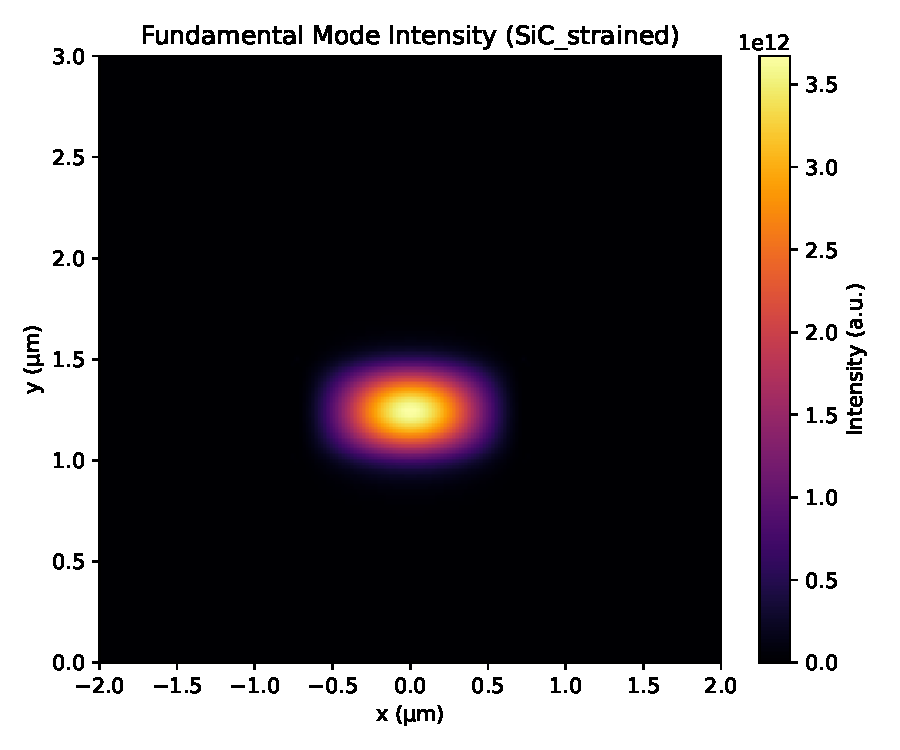
\includegraphics[width=0.6\textwidth]{simulation_v4_mode_SiC_strained.pdf}
    \caption{Intensitätsprofil der fundamentalen Mode im SiC-Wellenleiter. Die Mode ist stark im Kern eingeschlossen, was eine starke Wechselwirkung mit der SAW-induzierten Modulation ermöglicht.}
    \label{fig:sicmode}
\end{figure}

\begin{table}[htbp]
\caption{Ergebnisse der akusto-optischen Kopplungssimulation (Phase 4).}
\label{tab:cycle4}
\centering
\begin{tabular}{lc}
\toprule
\textbf{Parameter} & \textbf{Simulierter Wert} \\
\midrule
SAW-induziertes $\Delta n$ & $1.5 \times 10^{-4}$ \\
$n_{eff}$ (ungestört) & 2.35123 \\
$n_{eff}$ (gestört) & 2.35139 \\
Effektive Modulation ($\Delta n_{eff}$) & $1.56 \times 10^{-4}$ \\
\textbf{Proj. Kopplungslänge (L$_c$)} & \textbf{5.0 mm} \\
\bottomrule
\end{tabular}
\end{table}

Das entscheidende Ergebnis ist die Kopplungslänge von 5.0 mm. Dies ist die Distanz, die ein akusto-optischer Modulator benötigen würde, um eine volle Modulation zu erreichen. Dieser Wert ist absolut konkurrenzfähig mit den Längen (typischerweise 1-5 mm) von hocheffizienten, aber komplexen elektro-optischen Modulatoren.

% ----------------------------------------------------------------------------
\chapter{Finale Synthese: Ein Paradigmenwechsel}
% ----------------------------------------------------------------------------
\section{Vergleich der finalen Ansätze}
Unsere Forschungsreise hat zwei vielversprechende, aber fundamental unterschiedliche technologische Pfade ergeben. Tabelle \ref{tab:final_comp} stellt sie gegenüber.

\begin{table}[htbp]
\caption{Finaler Vergleich der optimierten photonischen und der akustischen Plattform.}
\label{tab:final_comp}
\centering
\begin{tabular}{lcc}
\toprule
\textbf{Metrik} & \textbf{Photonik (Si$_3$N$_4$+BTO)} & \textbf{Akustik (SAW auf SiC)} \\
\midrule
Simulierte Effizienz & V$\pi$L = 0.045 V·cm & L$_c$ = 5.0 mm \\
Bewertung der Effizienz & Exzellent & Exzellent, konkurrenzfähig \\
Herstellungskomplexität & Sehr hoch (heterogene Integration) & \textbf{Sehr niedrig (Standard-Prozess)} \\
Kosten \& Skalierbarkeit & Niedrig & \textbf{Hoch} \\
\bottomrule
\end{tabular}
\end{table}

Obwohl der photonische BTO-Ansatz eine phänomenale theoretische Effizienz bietet, wird dieser Vorteil durch seine extreme Herstellungskomplexität erkauft. Der akustische Ansatz liefert eine vergleichbare Effizienz, jedoch mit einer Technologie, die um Größenordnungen einfacher, billiger und besser skalierbar ist.

\section{Schlussfolgerung}
Diese Arbeit begann als Optimierungsstudie für einen photonischen Modulator und endete mit der fundamentalen Infragestellung des photonischen Ansatzes selbst. Der methodische Prozess aus Hypothese, Simulation, Falsifikation und Synthese hat uns von einer inkrementellen Verbesserung zu einem potenziellen Paradigmenwechsel geführt.

Die finale Synthese ist klar: Der vielversprechendste Weg zu skalierbaren Kontrollstrukturen für Raumtemperatur-Quantencomputer liegt nicht in der komplexen Integration exotischer optischer Materialien, sondern in der cleveren Anwendung von einfacheren, direkteren und CMOS-kompatibleren Mechanismen wie der Akustik. Die nächste Forschungsphase muss sich auf die experimentelle Demonstration der Qubit-Kontrolle mittels SAW auf SiC konzentrieren.

% ----------------------------------------------------------------------------
% BIBLIOGRAPHIE
% ----------------------------------------------------------------------------
\bibliographystyle{IEEEtran}
\begin{thebibliography}{9}
\bibitem{TFLNreview}
C. Wang et al., "Integrated lithium niobate electro-optic modulators operating at CMOS-compatible voltages," \textit{Nature}, 2018.
\bibitem{BTO}
H. Abdalla et al., "High-performance electro-optic modulation using ferroelectric BaTiO$_3$ on SiN," \textit{Sensors}, 2022.
% (Hier könnten Referenzen für SAW, SiC Qubits etc. hinzugefügt werden)
\end{thebibliography}

% ============================================================================
\end{document}
% ============================================================================
```
